% $Id: template.tex 11 2007-04-03 22:25:53Z jpeltier $

\documentclass{vgtc}                          % final (conference style)
%\documentclass[review]{vgtc}                 % review
%\documentclass[widereview]{vgtc}             % wide-spaced review
%\documentclass[preprint]{vgtc}               % preprint
%\documentclass[electronic]{vgtc}             % electronic version

%\documentclass{article}
\usepackage{ngerman}
\usepackage[T1]{fontenc}
\usepackage[utf8]{inputenc}

%% Uncomment one of the lines above depending on where your paper is
%% in the conference process. ``review'' and ``widereview'' are for review
%% submission, ``preprint'' is for pre-publication, and the final version
%% doesn't use a specific qualifier. Further, ``electronic'' includes
%% hyperreferences for more convenient online viewing.

%% Please use one of the ``review'' options in combination with the
%% assigned online id (see below) ONLY if your paper uses a double blind
%% review process. Some conferences, like IEEE Vis and InfoVis, have NOT
%% in the past.

%% Figures should be in CMYK or Grey scale format, otherwise, colour 
%% shifting may occur during the printing process.

%% These few lines make a distinction between latex and pdflatex calls and they
%% bring in essential packages for graphics and font handling.
%% Note that due to the \DeclareGraphicsExtensions{} call it is no longer necessary
%% to provide the the path and extension of a graphics file:
%% \includegraphics{diamondrule} is completely sufficient.
%%
\ifpdf%                                % if we use pdflatex
  \pdfoutput=1\relax                   % create PDFs from pdfLaTeX
  \pdfcompresslevel=9                  % PDF Compression
  \pdfoptionpdfminorversion=7          % create PDF 1.7
  \ExecuteOptions{pdftex}
  \usepackage{graphicx}                % allow us to embed graphics files
  \DeclareGraphicsExtensions{.pdf,.png,.jpg,.jpeg} % for pdflatex we expect .pdf, .png, or .jpg files
\else%                                 % else we use pure latex
  \ExecuteOptions{dvips}
  \usepackage{graphicx}                % allow us to embed graphics files
  \DeclareGraphicsExtensions{.eps}     % for pure latex we expect eps files
\fi%

%% it is recomended to use ``\autoref{sec:bla}'' instead of ``Fig.~\ref{sec:bla}''
\graphicspath{{figures/}{pictures/}{images/}{./}} % where to search for the images

\usepackage{microtype}                 % use micro-typography (slightly more compact, better to read)
\PassOptionsToPackage{warn}{textcomp}  % to address font issues with \textrightarrow
\usepackage{textcomp}                  % use better special symbols
\usepackage{mathptmx}                  % use matching math font
\usepackage{times}                     % we use Times as the main font
\renewcommand*\ttdefault{txtt}         % a nicer typewriter font
\usepackage{cite}                      % needed to automatically sort the references
\usepackage{tabu}                      % only used for the table example
\usepackage{booktabs}                  % only used for the table example
\usepackage{listings}
%% We encourage the use of mathptmx for consistent usage of times font
%% throughout the proceedings. However, if you encounter conflicts
%% with other math-related packages, you may want to disable it.


%% If you are submitting a paper to a conference for review with a double
%% blind reviewing process, please replace the value ``0'' below with your
%% OnlineID. Otherwise, you may safely leave it at ``0''.
\onlineid{0}

%% declare the category of your paper, only shown in review mode
\vgtccategory{Research}

%% allow for this line if you want the electronic option to work properly
\vgtcinsertpkg

%% In preprint mode you may define your own headline.
%\preprinttext{To appear in an IEEE VGTC sponsored conference.}

%% Paper title.

\title{MagicVR - 3D Models and Effects}

%% This is how authors are specified in the conference style

%% Author and Affiliation (single author).
%%\author{Roy G. Biv\thanks{e-mail: roy.g.biv@aol.com}}
%%\affiliation{\scriptsize Allied Widgets Research}

%% Author and Affiliation (multiple authors with single affiliations).
%%\author{Roy G. Biv\thanks{e-mail: roy.g.biv@aol.com} %
%%\and Ed Grimley\thanks{e-mail:ed.grimley@aol.com} %
%%\and Martha Stewart\thanks{e-mail:martha.stewart@marthastewart.com}}
%%\affiliation{\scriptsize Martha Stewart Enterprises \\ Microsoft Research}

%% Author and Affiliation (multiple authors with multiple affiliations)
\author{Jerome D. Pönisch\thanks{e-mail: jerome.poenisch@campus.lmu.de}\\ %
        \scriptsize 3D Models and Effects %
\and Michael Maier\thanks{e-mail: micahel.maier@campus.lmu.de}\\ %
     \scriptsize Gesture Recognition}

%% A teaser figure can be included as follows, but is not recommended since
%% the space is now taken up by a full width abstract.
%\teaser{
%  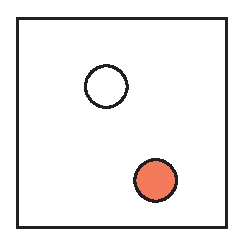
\includegraphics[width=1.5in]{sample.eps}
%  \caption{Lookit! Lookit!}
%}

%% Abstract section.
\abstract{
This documentation is about MagicVR - a virtual reality application developed
in OpenSG for the LRZ V2C in Garching supporting 3D-Gesture-Recognition and
Lerp-Animations. This document covers the part 3D-Gesture-Recognition.
} % end of abstract

%% ACM Computing Classification System (CCS). 
%% See <http://www.acm.org/about/class> for details.
%% We recommend the 2012 system <http://www.acm.org/about/class/class/2012>
%% For the 2012 system use the ``\CCScatTwelve'' which command takes four arguments.
%% The 1998 system <http://www.acm.org/about/class/class/2012> is still possible
%% For the 1998 system use the ``\CCScat'' which command takes four arguments.
%% In both cases the last two arguments (1998) or last three (2012) can be empty.

\CCScatlist{
  \CCScatTwelve{V2C}{Virtual Reality}{OpenSG}{Treemaps}{}
}

%\CCScatlist{
  %\CCScat{H.5.2}{User Interfaces}{User Interfaces}{Graphical user interfaces (GUI)}{};
  %\CCScat{H.5.m}{Information Interfaces and Presentation}{Miscellaneous}{}{}
%}

%% Copyright space is enabled by default as required by guidelines.
%% It is disabled by the 'review' option or via the following command:
% \nocopyrightspace

%%%%%%%%%%%%%%%%%%%%%%%%%%%%%%%%%%%%%%%%%%%%%%%%%%%%%%%%%%%%%%%%
%%%%%%%%%%%%%%%%%%%%%% START OF THE PAPER %%%%%%%%%%%%%%%%%%%%%%
%%%%%%%%%%%%%%%%%%%%%%%%%%%%%%%%%%%%%%%%%%%%%%%%%%%%%%%%%%%%%%%%%

\lstset{
    breaklines=true,
    tabsize=2,
    basicstyle=\ttfamily,
}


\begin{document}

%% The ``\maketitle'' command must be the first command after the
%% ``\begin{document}'' command. It prepares and prints the title block.

%% the only exception to this rule is the \firstsection command
\firstsection{Introduction}

\maketitle

%% \section{Introduction} %for journal use above \firstsection{..} instead
In this documentation the concept and implementation of MagicVR gestures will be
explained. MagicVR is a virtual reality application which was developed in C++
and OpenSG in order to run in the V2C mixed reality cave of the LRZ in Garching,
Munich. It\rq{}s main feature is a 3D-Gesture-Recognition opening a whole world
of interaction possibilities using only the wand (or any tracker) in a 3D
tracking system.

\section{Concept}

MagicVR was developed in a cooperation between Jerome Pönisch and Michael Maier. This paper will be focused on the 3D Art and FractTime-Animation effects done by Jerome Pönisch while Michaels\rq{}s paper will be focused on the 3D-Gesture-Recognition.
This section shall introduce in the general concept of MagicVR and the effects and animation part.

\subsection{The idea behind MagicVR}

The main idea of MagicVR is introducing the 3D-Gesture-Recognition module in a playful environment using important features of a virtual environment. A user/player should be animated to use 3D-Gestures as interesting interaction technique rather than pushing buttons. The virtual environment should help to gain the user/player\rq{}s interest and make him feel comfortable while experiencing the mixed reality world. As User-Feedback it was decided to focus on animations and movements within the scene.

\subsection{FractTime-Animations}

In order to make movements easier to implement and control a framework was implemented based on the idea of Vector Lerp, FractTime and Coroutines from Unity and C\#.
\begin{description}
 \item{\textbf{Lerp}} is a commonly used short term standing for \lq\lq{}linear interpolation\rq\rq{}. The concept of a Vector.Lerp in Unity and C\# takes an original vector and a target vector and makes a linear interpolation between those two vectors using an interpolation factor from 0 to 1.
 
 \item{\textbf{FracTime}} is used as the interpolation factor in our framework. It devides the already animated time by the target duration of the animation providing a factor between 0 and 1.
 
 \item{\textbf{Coroutines}} are used in Unity to run multible routines at the same time which makes it easier to control them individually. The difference to c++ is, that multithreading is more trivial in C\#.
 \end{description}
 
 Those two concepts were used in combination to write our own FractTime-Animations framework.\\
 
 \subsection{Advantages of FracTime Animations}
 The advantages of using our animation framework are among others:
 \begin{description}
 \item{\textbf{Trustability}} Destination and Target values of vectors, colors etc. are clear defined and thereby no \lq\lq{}surprises will happen during animations\rq\rq{}
 \item{\textbf{Controlability}} Since all animations are placed and controlled in one main container and subcontainers, each animation can be started and stopped individually.
 \item{\textbf{FPS-Stability}} Since the animations are based on the FracTime, which is based on the delta time between frames, and not e.g. the translation distance animations will allways take the same time independent of the FPS given by the render system.
 \end{description}

\section{Implementation}

In this section some implementation details will be given for the animations and effects.

\subsection{Environment}
An important part in the user experience with mixed and virtual reality plays the virtual environment. Here a combination of a skybox and an environment 3D-model was used to get the most out of the V2C cave regarding to immersion. The skybox image was rendered using an HDRI image and a self written hdri to image converter in Blender 3D.

\begin{figure}[!ht]
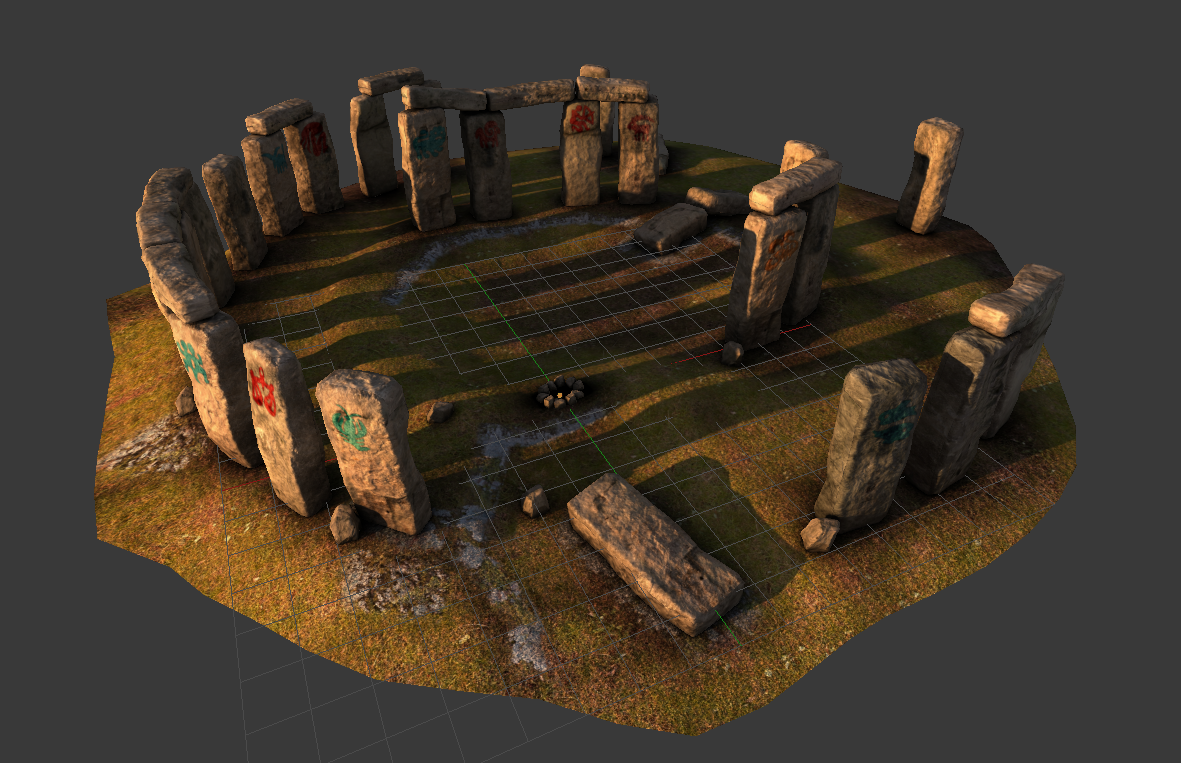
\includegraphics[width=0.4\textwidth]{pictures/stonehenge.png}
\caption{Stonehenge by ruslans3d is licensed under CC Attribution https://sketchfab.com/models/37cfc2bb99944703b5d57ea281030ca6}
\end{figure}

\begin{figure}[!ht]
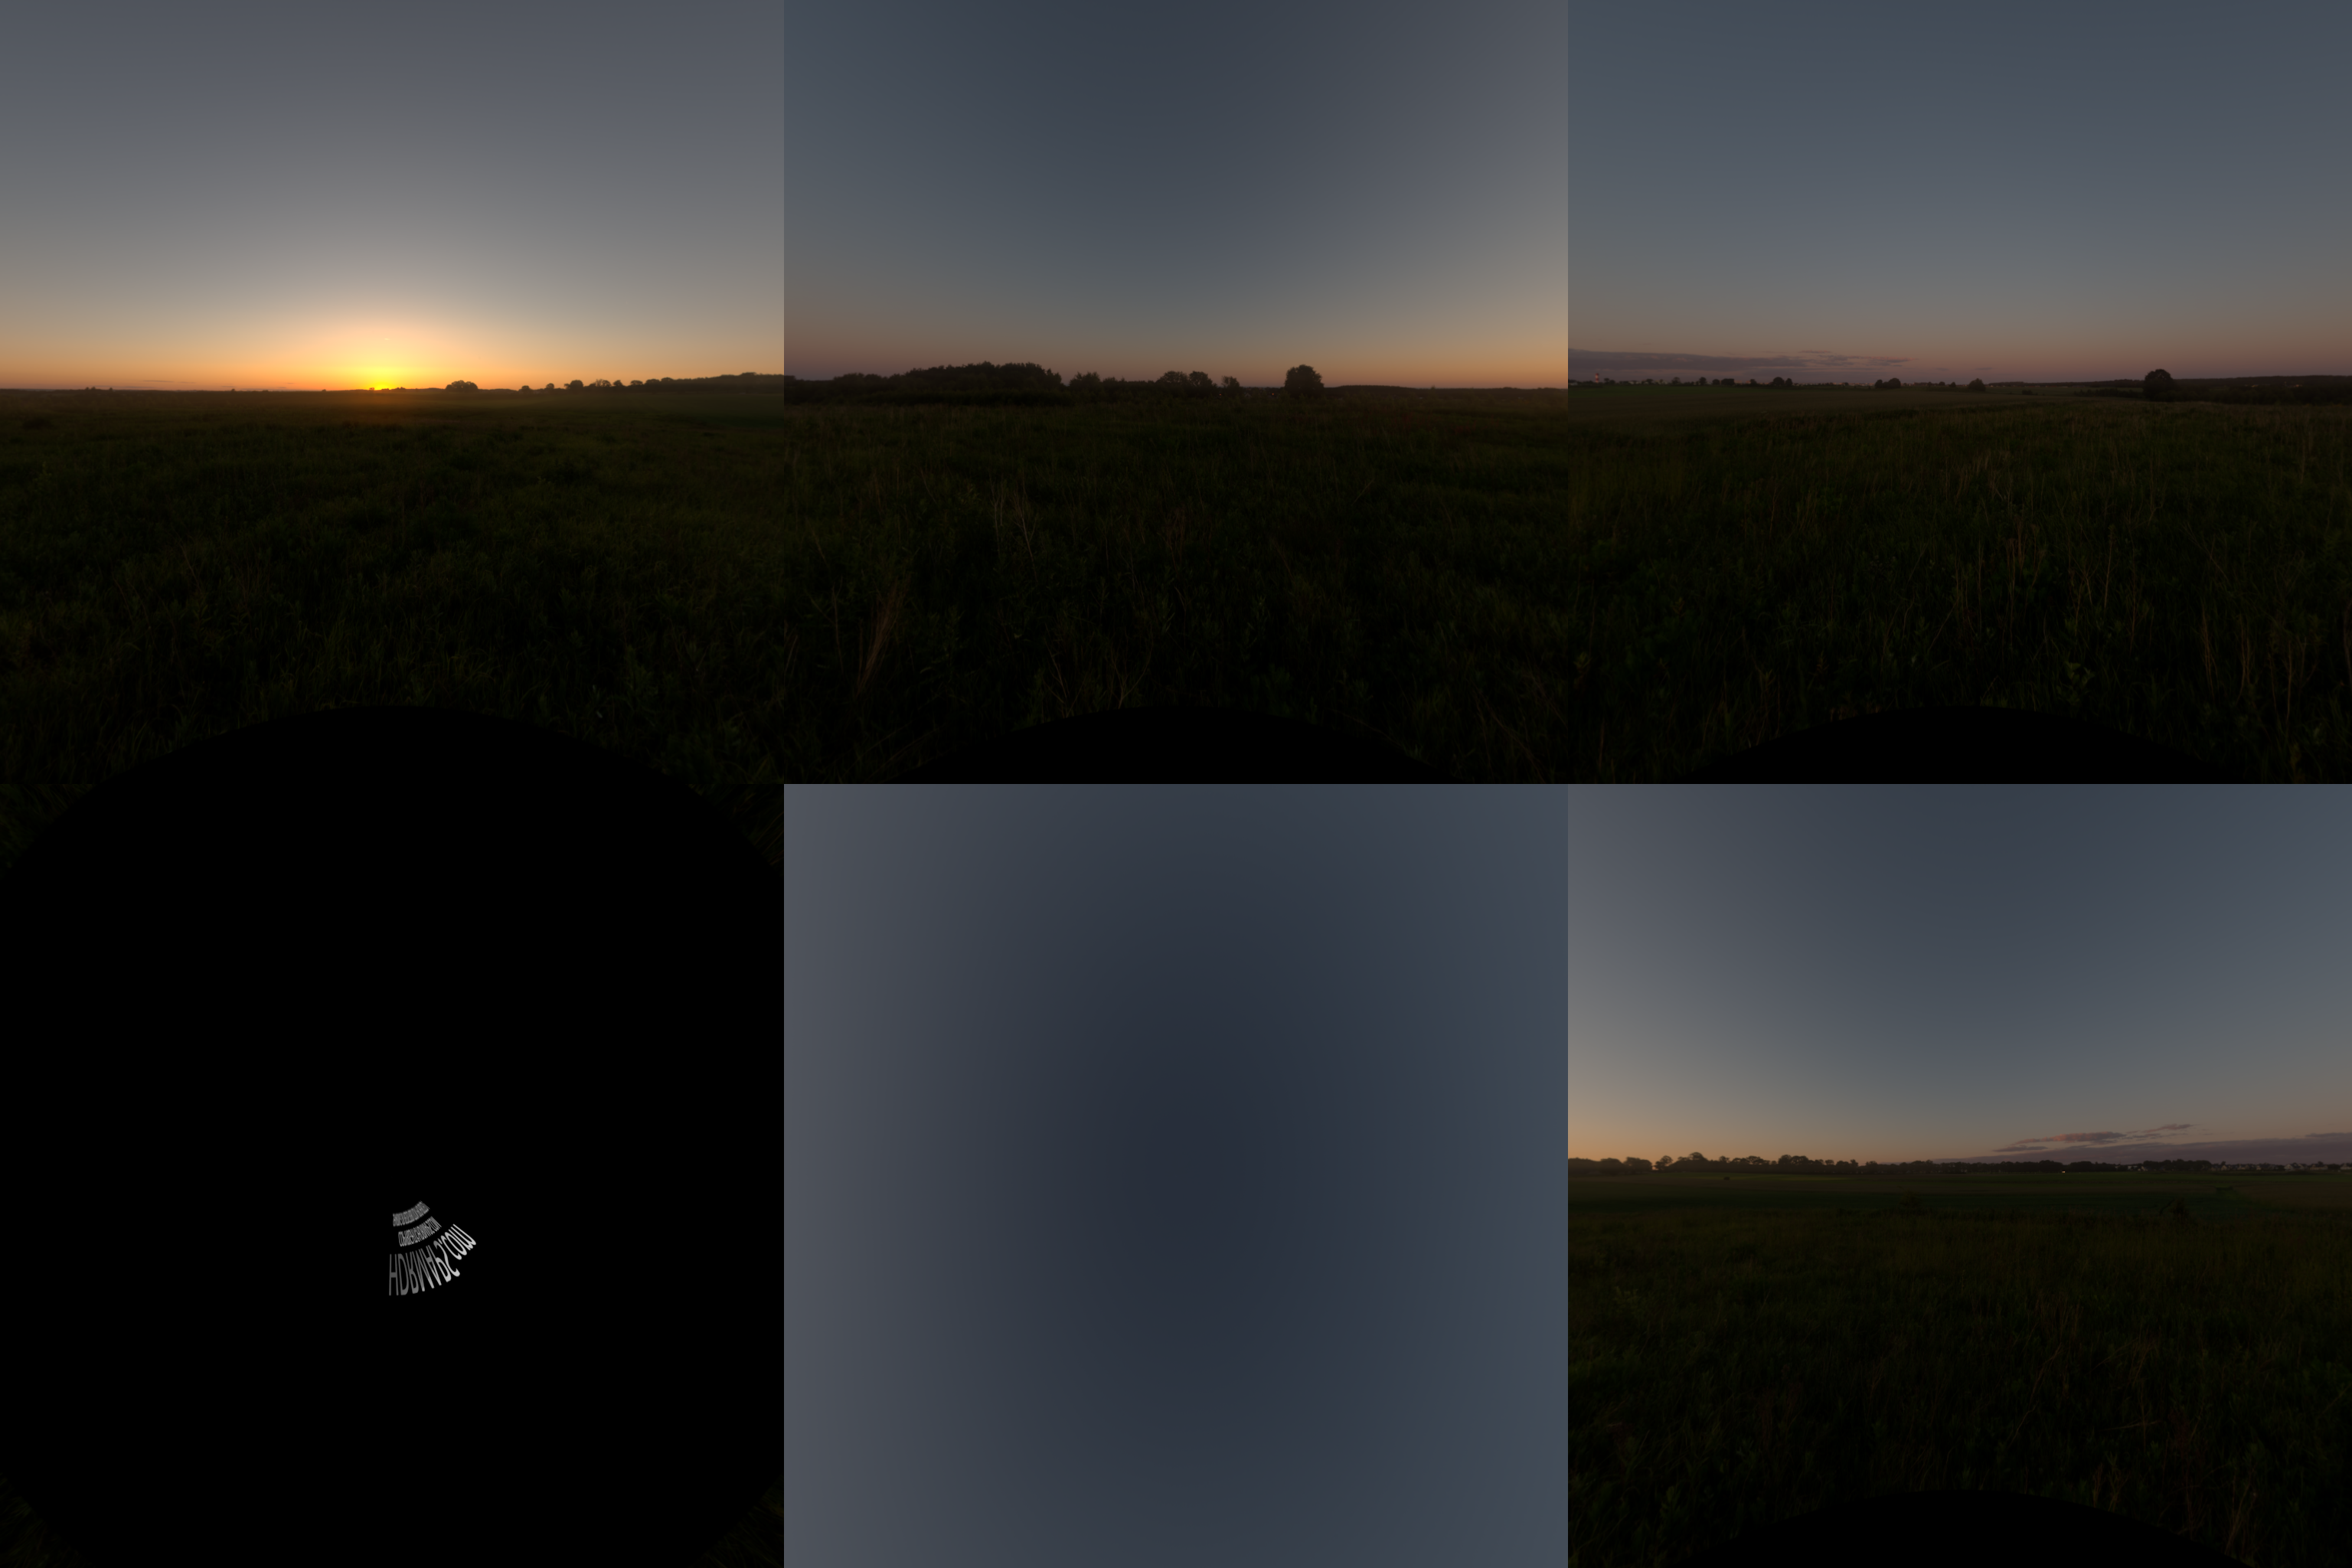
\includegraphics[width=0.4\textwidth]{pictures/EnvMap_cube_1024.png}
\caption{Source: https://hdrmaps.com }
\end{figure}

\vfill

\begin{lstlisting}[caption={Implementing the Skybox}][H!]
SkyBackgroundUnrecPtr loadBackground(Resolutions skyboxResolution) {
   
 std::string bgImageFilePath = Path_to_Skybox_image;

 ImageUnrecPtr mainImage = ImageFileHandler::the()->read(bgImageFilePath.c_str());

 /**
 * Create empty images as destinations for subimage */
 ImageUnrecPtr imgFront = ImageBase::create();
 ImageUnrecPtr imgBack = ImageBase::create();
 ImageUnrecPtr imgLeft = ImageBase::create();
 ImageUnrecPtr imgRight = ImageBase::create();
 ImageUnrecPtr imgTop = ImageBase::create();
 ImageUnrecPtr imgBottom = ImageBase::create();

 /**
  * Easier to change Skybox Images by croping them out
  * at runtime directly from the CubeMap Image exported from Blender
  *
  * Blender exports the environment maps in the format:
  *
  * Left   | Back | Right
  * Bottom | Top  | Front
  *
  * While subImage reads 
  * - offX from left to right
  * - offY from bottom to top */
 mainImage->subImage(2 * res, 0  , 0, 
   res, res, 1, 
   imgFront);
 mainImage->subImage(res , res, 0, 
   res, res, 1,
    imgBack);
 mainImage->subImage(0  , res, 0, 
   res, res, 1, 
   imgLeft);
 mainImage->subImage(2 * res, res, 
   0, res, res, 1, 
   imgRight);
 mainImage->subImage(res, 0  , 0, 
   res, res, 1, 
   imgTop);
 mainImage->subImage(0 , 0  , 0, 
   res, res, 1, 
   imgBottom);

    /**
     * Create Textures and set image to cropped images */
    TextureObjChunkUnrecPtr texFront = TextureObjChunk::create();
    texFront->setImage(imgFront);

    TextureObjChunkUnrecPtr texBack = TextureObjChunk::create();
    texBack->setImage(imgBack);

    TextureObjChunkUnrecPtr texLeft = TextureObjChunk::create();
    texLeft->setImage(imgLeft);

    TextureObjChunkUnrecPtr texRight = TextureObjChunk::create();
    texRight->setImage(imgRight);

    TextureObjChunkUnrecPtr texTop = TextureObjChunk::create();
    texTop->setImage(imgTop);

    TextureObjChunkUnrecPtr texBottom = TextureObjChunk::create();
    texBottom->setImage(imgBottom);

    /**
     * Create Skybox and set textures */
    SkyBackgroundUnrecPtr skyBG = SkyBackground::create();
    skyBG->setFrontTexture(texFront);
    skyBG->setBackTexture(texBack);
    skyBG->setLeftTexture(texLeft);
    skyBG->setRightTexture(texRight);
    skyBG->setTopTexture(texTop);
    skyBG->setBottomTexture(texBottom);

    return skyBG;
}

\end{lstlisting}

\subsection{Animations}

While the \emph{Lerp} and the \emph{FracTime} was easy to implement in c++, for the \emph{Coroutines} had to be found another solution. To make things easy an animation holder was implemented, controlling all animations of the scene in one place.

\begin{lstlisting}[breaklines=true]
void Scene::update(OSG::Time dTime) {
 _animations.animate(dTime);
}
\end{lstlisting}

The framework which was implemented uses two main animation classes \lq\lq{}ParallelAnimation\rq\rq{} and \lq\lq{}SequentialAnimation\rq\rq{} defining as the name lets guess already whether contained animations shall be performed simultaneously or sequentially. So it\rq{}s easy to guess that the Scene::\_animations is a ParallelAnimation animating all contained animations at the same time.
\begin{lstlisting}[breaklines=true, caption={ParallelAnimation::animate}]
void ParallelAnimation::animate(OSG::Time dTime) {
 for (auto animation : _animations) {
  animation->animate(dTime);
 }
 removeStoppedAnimations();
 if (_stopIfNoAnimations && _animations.empty()) {
  stop();
 }
}
\end{lstlisting}

\begin{lstlisting}[breaklines=true, caption={SequentialAnimation::animate}]
void SequentialAnimation::animate(OSG::Time dTime) {
 if (_stopIfNoAnimations && _animations.empty()) {
  stop();
 } else {
  _animations.front()->animate(dTime);
  if (_animations.front()->isStopped()) {
   _animations.pop();
   if (_stopIfNoAnimations && _animations.empty()) {
    stop();
   }
  }
 }
}
\end{lstlisting}

Then there are some animation wrappers like \lq\lq{}EaseInAnimation\rq\rq{}, \lq\lq{}EaseOutAnimation\rq\rq{} and \lq\lq{}BezierAnimation\rq\rq{} allowing to implement completely ease controlled animations and even a forward-backwards animation as seen in the example below:
\begin{lstlisting}[breaklines=true, caption={BezierAnimation::animate}]
void BezierAnimation::animateFracTime(OSG::Time fracTime) {
 _animation->animate(_bezier.atPercentage(fracTime).y());
}
\end{lstlisting}

Finally there are the actual animation performing the before mentioned Lerp on Vectors \lq\lq{}TranslationAnimation\rq\rq{} and \lq\lq{}ScaleAnimation\rq\rq{} as seen in the example below:
\begin{lstlisting}[breaklines=true, caption={TranslattionAnimation::animate}]
void TranslationAnimation::animateFracTime(OSG::Time fracTime) {
 Vec3f _movement = _destination - _start;
 _trans->setTranslation(_start + _movement * fracTime);
}
\end{lstlisting}

\subsection{Effects}
Based on this animations framework the effects and user feedback was implemented using for example a TranslationAnimation and a ScaleAnimation wrapped in a ParallelAnimation with repetition enabled:
\begin{lstlisting}[breaklines=true, caption={BubbleAnimationsNode::animate}]
void BubbleAnimationsNode::addAnimations() {
 for (const auto &data : _bubbleDatas) {
  _animations.add(std::shared_ptr<Animation>(
   new ParallelAnimation{
    std::shared_ptr<Animation>(
     new TranslationAnimation(
      data.transformation,
      OSG::Vec3f(0, 1, 0),
      3 * data.data, true)),

    std::shared_ptr<Animation>(
     new ScaleAnimation(
      data.transformation,
      OSG::Vec3f(0, 0, 0),
      3 * data.data, true))
     }
  ));
 }
}
\end{lstlisting}


\section{Use cases and User Guide}
In this section we come to some use cases of the FracTime animations, the user gameplay and instruction of MagicVR.

TODO! pictures\\
\begin{figure}[!ht]
\includegraphics[width=0.4\textwidth]{pictures/scene-overview-1.jpg}
\includegraphics[width=0.4\textwidth]{pictures/scene-overview-2.jpg}
\caption{Scene Overview}
\end{figure}

\subsection{Element Stones}
In the virtual scene are placed some columns with \lq\lq{}Elementary Stones\rq\rq{}. They have different symbols as texture representing the according element and at the same time the 3D-Gesture which has to be performed to call this element. Those \lq\lq{}Elementary Stones\rq\rq{} can also be used to practice and get used to the 3D-Gestures.

If the a 3D-Gestures of one of the elements is correctly recognized, a BubbleAnimation as explained before starts to run, letting the user know, which element he activated.

\subsection{Shooting Elements}
If practiced enough, the user can feel free to move on to shoot elements. This is done by a combination of 3D-Gestures:
\begin{itemize}
\item{1.} Make a circle gesture: This activates the \lq\lq{}Shoot Mode\rq\rq{}. You will see this as there should appear a neutral ball at the top of your wand.
\item{2.} Make the element gesture of your wish: This calls the element. You should see that the ball at the top of your wand changes into the according element - equal to the element bubbles you saw on the elementary stones.
\item{3.} Make a multiplication gesture: This allows later on to shoot multiple element bubbles at once according to how many times you use this gesture. You should notice, that the ball at the top of the wand grows according to the multiplication.
\item{4.} Shoot the element using the shoot gesture. The element bubbles will shoot out of your wand searching its way to the according interaction. If you had multiplication done, you will see the ball shrink while shooting multiple bubbles.
\end{itemize}

\subsubsection{Fire and Water}
TODO! pictures\\
\begin{figure}[!ht]
\includegraphics[width=0.4\textwidth]{pictures/fire-gesture.jpg}
\includegraphics[width=0.4\textwidth]{pictures/water-gesture.jpg}
\caption{Fire and Water gestures}
\end{figure}

Element bubbles of the type water and fire will have their target on the fireplace located at the left side of the scene. Fire bubbles make the fire grow bigger while water will shrink it down.

\subsubsection{Lightning}
TODO! picture\\
\begin{figure}[!ht]
\includegraphics[width=0.4\textwidth]{pictures/lightning-gesture.jpg}
\caption{Lightning gesture}
\end{figure}

Element bubbles of the type Lightning will have their target at the lantern placed in the front part of the scene. As it is hit by the bubbles, the scene will be lit more and more.

\subsubsection{Wind}
TODO! picture\\
\begin{figure}[!ht]
\includegraphics[width=0.4\textwidth]{pictures/wind-gesture.jpg}
\caption{Wind gesture}
\end{figure}
TODO! description\\

\section{Outlook}

The implemented animation framework makes it easy to implement further animation types and more complex movements while they stay very control- and adjustable. There are multiple further ways how and where this animation framework could be applied e.g. animating not only Vectors but also materials, colors, transparency etc.\\

Since there wasn\rq{}t enough time to finish all our ideas, the interactions for lightning and wind bubbles was not completely implemented. Hitting the lantern with lightning bubbles should have lit up the scene bit by bit as if the light was trapped inside the lantern. The wind gesture should have activated a kind of manipulation mode in combination with a second gesture setting a direction. With this combination it should have been possible to move the lantern around in the scene in order to light up different parts of the scene.\\

Also because of the lack of time there was no opportunity to implement a better user guidance. Our idea would have been to implement a little fairy which gives hints about interaction possibilities and demonstrates according gestures by flying them in front of the user.



%\bibliographystyle{abbrv}
\bibliographystyle{abbrv-doi}
%\bibliographystyle{abbrv-doi-narrow}
%\bibliographystyle{abbrv-doi-hyperref}
%\bibliographystyle{abbrv-doi-hyperref-narrow}

\bibliography{template}
\end{document}
